\documentclass{article}
\usepackage{ee105}

%% Makes figure labels bold
\usepackage[labelfont=bf]{caption}

\begin{document}

%% Prevent headings on the first page, since we're not using \maketitle
\thispagestyle{plain}

%% Standard header. Title of the lab goes here.
\lab{10}{Differential Amplifiers}

\section{Objective}

Differential amplifiers are designed to amplify the difference between two signals. Differential amplifiers are thereby able to reduce noise that is common to both inputs, only amplifying the differential signal that we're interested in. We can quantify the differential-mode versus common-mode gain in a quantity called the common-mode rejection ratio (CMRR). Differential amplifiers also lend themselves to use in feedback, though we will not explore that usage in this lab. A typical differential amplifier with a single-ended output that you are familiar with is the op-amp.

\section{Materials}

For this lab, assume all NPN transistors are identical 2N3904 BJTs and all PNP transistors are identical 2N3906 BJTs.

\begin{table}[!htb]
  \begin{center}
    \begin{tabular}{|c|c|} \hline
      Component & Quantity \\\hline
      LM741 op-amp & 1 \\
      2N3904 NPN BJT & 4 \\
      2N3906 PNP BJT & 2 \\
      \unit{1}{\kilo\ohm} resistor & 2 \\
      \unit{5.1}{\kilo\ohm} resistor & 2 \\
      \unit{10}{\kilo\ohm} resistor & 2 \\
      \unit{0.1}{\micro\farad} capacitor & 1 \\\hline
    \end{tabular}
    \caption{Components used in this lab}
    \label{components}
  \end{center}
\end{table}

\begin{table}[!htb]
  \begin{center}
    \begin{tabular}{|c|c|c|c|} \hline
      Component & $I_S$ (A) & $V_A$ (V) \\\hline
      2N3904 NPN BJT & $6.734 \times 10^{-15}$ & $74.03$ \\
      2N3906 PNP BJT & $1.41 \times 10^{-15}$ & $18.7$ \\\hline
    \end{tabular}
    \caption{Transistor properties}
    \label{params}
  \end{center}
\end{table}

\section{Procedure}

\subsection{Generating a differential signal}

Before building a differential amplifier, we'd like to be able to generate a differential signal. This requires inverting an analog signal. One way we can do this is by using an op-amp in negative feeback, as shown in Figure \ref{inverter}.

\begin{figure}[!htb]
  \input inverter
  \centerline{\box\graph}
  \caption{Inverting amplifier}
  \label{inverter}
\end{figure}

\begin{enumerate}
  \item Construct the circuit in Figure \ref{inverter}. Use the LM741 op-amp. The pin layout for the LM741 op-amp is in Figure \ref{LM741}. \note{If your LM741 doesn't have a notch as shown in the figure, check for a small dot. This dot labels pin 1.}

\begin{figure}[!htb]
  \centering
  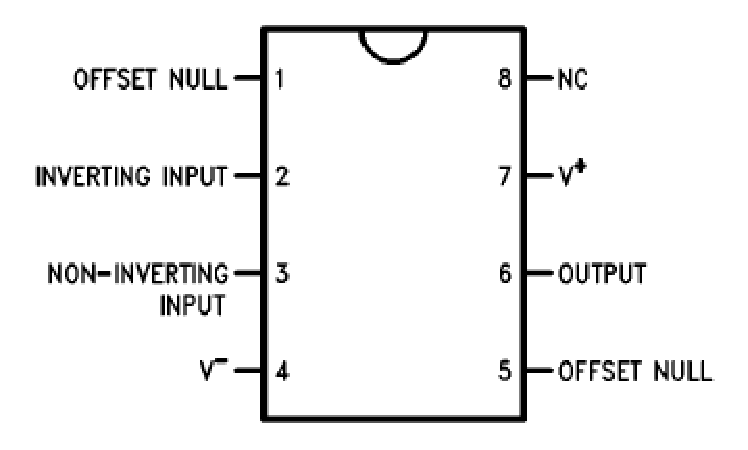
\includegraphics[width=0.35\textwidth]{LM741.eps}
  \caption{LM741 pin layout}
  \label{LM741}
\end{figure}

  \item Apply a \unit{30}{\milli\volt} amplitude, \unit{1}{\kilo\hertz} sine wave to the input. Display the input and output on the oscilloscope. The output should be the inverse of the input.
\end{enumerate}

\subsection{Differential pair with resistive load}

\begin{enumerate}
  \item Construct the circuit in Figure \ref{diff} using 2N3904 transistors for the NPN BJTs. Use $R_1 = \unit{10}{\kilo\ohm}$, $R_2 = R_3 = \unit{5.1}{\kilo\ohm}$, and $V_{CC}=\unit{9}{\volt}$. This is the same circuit you analyzed in the prelab.

\begin{figure}[!htb]
  \input diff
  \centerline{\box\graph}
  \caption{Differential pair with resistive load}
  \label{diff}
\end{figure}

  \item Ground the inputs and measure $I_{C1}$, $I_{C2}$, $I_{C3}$, and $V_{OUT,DC}$. How do these values compare to what you'd expect from hand calculations?
  \item Apply a \unit{30}{\milli\volt} amplitude, \unit{1}{\kilo\hertz} sine wave to $v_{in+}$ and ground $v_{in-}$. Use the oscilloscope to display the input waveform at $v_{in+}$ and the output waveform at $v_{out+}$ and sketch the result. If the input signal is noisy, use the averaging feature of the oscilloscope to get a more accurate result.
  \item Use the oscilloscope to measure the peak-to-peak voltages of $v_{in+}$ and $v_{out+}$.
  \item Use the oscilloscope to display $v_{out+}$ and $v_{out-}$. Do they appear as you'd expect?
  \item Use the oscilloscope to display $v_{out+} - v_{out-}$. Measure the peak-to-peak voltage of the signal and calculate the differential gain of the circuit. Does this match the gain you calculated in the prelab?
  \item Apply a \unit{30}{\milli\volt} amplitude, \unit{1}{\kilo\hertz} sine wave to both $v_{in+}$ and $v_{in-}$. Use the oscilloscope to display the output waveform at $v_{out+}$ and $v_{out-}$. What do you see at the output? Why?
  \item Use the inverting amplifier you built to apply a \unit{20}{\milli\volt} amplitude, \unit{1}{\kilo\hertz} differential sine wave to the inputs (that means a \unit{10}{\milli\volt} amplitude sine wave to $v_{in+}$ and the inverted sine wave to $v_{in-}$). Measure the peak-to-peak voltage of the differential input and output with the oscilloscope. Does the gain match your prelab calculations? Does it match the gain you observed in step 3.2.6?

\end{enumerate}

\subsection{Differential pair with active load}

\begin{figure}[!htb]
  \input activediff
  \centerline{\box\graph}
  \caption{Differential pair with active load}
  \label{activediff}
\end{figure}

\begin{enumerate}
  \item Construct the circuit in Figure \ref{activediff} using 2N3904 transistors for the NPN BJTs and 2N3906 transistors for the PNP BJTs. Use $R_1 = \unit{10}{\kilo\ohm}$ and $V_{CC}=\unit{9}{\volt}$.
  \item Apply a \unit{30}{\milli\volt} amplitude, \unit{1}{\kilo\hertz} sine wave to $v_{in+}$ and ground $v_{in-}$. Use the oscilloscope to display the output waveform at $v_{out}$ and sketch the result. Why isn't the output sinusoidal?
  \item We'd like to reduce $R_{out}$ by loading the amplifier with a small resistor. Attach a load to the amplifier as shown in Figure \ref{activediffload}. Use $C_L = \unit{0.1}{\micro\farad}$ and $R_L = \unit{5}{\kilo\ohm}$.

    \begin{figure}[!htb]
      \input activediffload
      \centerline{\box\graph}
      \caption{Differential pair with reduced output resistance}
      \label{activediffload}
    \end{figure}

  \item Calculate the differential gain for the amplifier with the new load resistance.
  \item Apply a \unit{20}{\milli\volt} amplitude, \unit{1}{\kilo\hertz} sine wave to $v_{in+}$ and ground $v_{in-}$. Use the oscilloscope to display $v_{in+}$ and $v_{out}$. Sketch $v_{out}$. What is the measured differential gain of the circuit? How does this compare with your hand calculations? Does the gain match the differential gain you measured in step 3.2.6? Should it?
\end{enumerate}

\subsection{SPICE Analysis}

\begin{enumerate}
  \item Write a netlist for the circuit in Figure \ref{diff}. Apply a differential input of amplitude \unit{20}{\milli\volt}, frequency \unit{1}{\kilo\hertz} as you did in step 3.2.8. \hint{Generate a \unit{20}{\milli\volt} amplitude, \unit{1}{\kilo\hertz} sine wave and use dependent sources to generate the non-inverted and inverted \unit{10}{\milli\volt} amplitude sine waves}.
  \item Use SPICE to find $I_{C1}$, $I_{C2}$, $I_{C3}$, and $V_{OUT,DC}$. Compare these values with your calculations from the prelab and measurements in lab.
  \item Plot the differential input and differential output signals in Awaves. Print the plot and attach it to your lab worksheet. Use the plot to calculate the gain. Does it match your hand calculations? Does it match your measurements?
\end{enumerate}

\end{document}